\chapter{基于PCDM的极化SAR图像舰船目标检测}
\label{cha:PCDM}

\section{引言}
\label{sec:chap4:sec1}
在第\ref{cha:PWF}章与第\ref{cha:LMM}章,我们实现了基于PWF与LMM模型的舰船检测算法,这两种方法都是
基于图像强度信息进行统计建模以区分舰船目标与背景杂波。然而基于强度或幅值的方法易受海况的影响从而
对海杂波的统计建模不够精确,使得检测性能下降。在本章中我们实现了基于极化协方差差异矩阵的极化SAR
舰船目标检测方法。在极化SAR图像目标检测中,舰船目标点的邻域像素提供了丰富的空间相干信息,极化协方
差矩阵主要度量了待检测像素与其3x3邻域像素的协方差矩阵的差异,基于该极化差异矩阵,我们应用了SPAN检测器得到了
粗略的舰船检测结果。同时我们将PCDM矩阵进行分解提取了新的极化特征基础船高(PSH),通过此极化特征结合SPAN检测器
的初步结果得到最终的检测二值图像。




\section{PCDM理论背景}
\label{sec:chap4:sec2}
\subsection{极化SAR散射表征与SPAN理论}
    通常散射矩阵被用来描述目标散射体的极化信息。在使用水平与垂直极化基的典型极化SAR系统中,复散射矩阵
    定义为如下的形式,其中$S_{HH}$代表了水平发射水平接收的极化信息,当满足互易性的条件时,$S_{HV}=S_{VH}$此时复散射
    矩阵可用三维的复散射矢量$k$式\ref{equ:chap4:kvector}来表示。

    \begin{equation}
        \label{equ:chap4:Smatrix}
        S = \left[ {\begin{array}{*{20}{c}}
        {{S_{HH}}}&{{S_{HV}}}\\
        {{S_{VH}}}&{{S_{VV}}}
        \end{array}} \right]
    \end{equation}

    \begin{equation}
        \label{equ:chap4:kvector}
        k = [{S_{HH}},\sqrt 2 {S_{HV}},{S_{VV}}]
    \end{equation}

    将散射矩阵进行变换可以得到更多散射体的极化信息,如式\ref{equ:chap4:cov}为散射矢量对应的3x3极化协防差矩阵。在该式
    中$\left\langle {} \right\rangle$代表在空间域上求平均,$\left| {} \right|$代表幅度值,$H$代表共轭转置。

    \begin{equation}
        \label{equ:chap4:cov}
        [C] = \left\langle {k \cdot {k^H}} \right\rangle  = \left[ {\begin{array}{*{20}{c}}
        {{C_{11}}}&{{C_{12}}}&{{C_{13}}}\\
        {{C_{21}}}&{{C_{22}}}&{{C_{23}}}\\
        {{C_{31}}}&{{C_{32}}}&{{C_{33}}}
        \end{array}} \right]
    \end{equation}

    在极化协方差矩阵$C$中,将对角线元素之和定义为为后向散射总功率即SPAN,如式\ref{equ:chap4:span}所示。还可以对
    极化协方差矩阵进行分解如式\ref{equ:chap4:decompose}所示,其中$\lambda_i$为极化协方差矩阵特征值,$v_i$为$\lambda_i$对应的
    特征向量。
    \begin{equation}
        \label{equ:chap4:span}
        {\rm{SPAN}} = {C_{11}} + {C_{22}} + {C_{33}}
    \end{equation}
    \begin{equation}
        \label{equ:chap4:decompose}
      C = \sum\limits_{i = 1}^3 {{\lambda _i}({v_i} \cdot {v_i}^H)} 
    \end{equation}

    \subsection{极化协方差差异矩阵}
    在计算机视觉领域,LBP特征(局部二值模式)用来描述光学图像中的纹理特征,被广泛应用于人脸检测与目标识别。
    LBP特征是将一个3x3区域内的中心像素值与邻域像素值做比较,并将得到的八位二进制结果重新排列构成一新二进制数值,
    该数值作为此区域中心像素的LBP特征值,如式\ref{equ:chap4:LBP}所示,其中$g_i$表示邻域内第i个像素的灰度值
    $g_c$为中心像素灰度值。$x_c, y_c$表示中心图像坐标。

    \begin{equation}
        \label{equ:chap4:LBP}
        [LB{P_{({x_c},{y_c})}} = \sum\limits_{i = 0}^{n - 1} {{2^{is({g_i} - {g_c})}}} ,s(x) = \left\{ {\begin{array}{*{20}{c}}
        1&{x \ge 0}\\
        0&{x < 0}
        \end{array}} \right.
    \end{equation}

    类比光学图像中的LBP特征,在极化SAR图像中,采用极化协方差矩阵来描述图像的极化信息。在光学图像中像素的灰度值
    可以通过R、G和B三个通道进行计算得到,而极化协防差矩阵也包含了极化SAR图像的HH、HV和VV通道的信息,但区别是灰度值
    只含有图像的一个特征,而极化协防差矩阵包含了九个极化特征,因此对此模型改进引入极化协方差差异矩阵(PCDM)

    定义${C^{(x,y)}}$为极化SAR图像索引为$x,y$像素处的极化协防差矩阵,接下来计算其3x3邻域上的协方差累积差异$P^{(x,y)}$,
    称$P^{(x,y)}$为极化SAR图像$x,y$处的极化协方差差异矩阵,如式\ref{equ:chap4:PCDM}所示,其中$C_{m,n}^{(i,j)}$为
    图像索引$i,j$处协方差矩阵的第$(m,n)$个元素。

    \begin{equation}
        \label{equ:chap4:PCDM}
        P_{m,n}^{(i,j)} = \sum\limits_{\Delta i =  - 1,\Delta j =  - 1}^1 {\left| {C_{m,n}^{(i,j)} - C_{m,n}^{(i + \Delta i,j + \Delta j)}} \right|}
    \end{equation}

    \begin{figure}[H] % use float package if you want it here
      \centering
      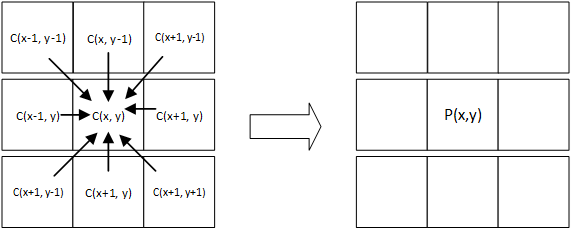
\includegraphics[width=0.9\textwidth]{PCDMCal.png}
      \caption{PCDM矩阵计算示意图}
      \label{fig:chap4:PCDM}
    \end{figure}   
  \section{基于PCDM的舰船目标检测算法}
      前三节我们描述了PCDM可以综合利用待检测像素与其邻域的像素的相干信息,在此基础上我们
      提出了基于极化协方差差异矩阵的舰船检测方法。对于输入的原始极化SAR图像数据,我们首先计算
      每个像素的极化协防差矩阵,然后按照式\ref{equ:chap4:PCDM}计算每个像素对应的极化协方差差异
      矩阵。得到极化协方差差异矩阵$\bf{P}$后,首先对$\bf{P}$矩阵应用SPAN检测器,即当$\rm{SPAN}_{\bf{P}}$>$T_{\rm{SPAN}}$
      时,认定该检测像素为舰船目标像素。

      对PCDM矩阵应用SPAN检测器后输出初步检测结果,为了提升检测的精度,我们进一步提取极化
      协方差差异矩阵的极化特征来区分舰船目标与背景杂波。通常SAR图像目标散射特性可以用极化特征来描述,例如
      极化分解,极化反对称性等极化特征。在文献\ref{}中提出了pedestal height特征来描述目标的散射特性,
      该极化特征实质上等价于极化协方差矩阵最小特征值与最大特征值的比值。实验表明低海况的背景杂波与方位向模糊像素的
      pedestal height极化特征值比真实的舰船像素要低很多。
       \begin{equation}
          {\rm{PSH = }}\frac{{\left| {{\lambda _3}} \right|}}{{\left| {{\lambda _1}} \right| + \left| {{\lambda _2}} \right|}}
      \end{equation}

      基于极化协方差差异矩阵我们重新计算这些极化特征,并将第二特征值考虑在内,新的极化特征命名为pedestal ship height(PSH)。对于提取的PSH极化特征,应用适当
      的检测阈值,来区分舰船目标与背景杂波像素。整个算法的流程如图\ref{fig:chap4:PCDMalg}所示,算法描述如算法\ref{alg:chap4:PCDMALG}所示

    \begin{figure}[H] % use float package if you want it here
      \centering
      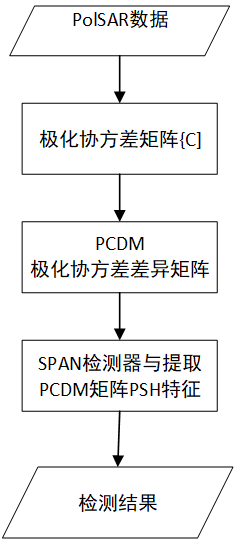
\includegraphics[height=0.5\textwidth]{PCDMalg.png}
      \caption{PCDM检测流程示意图}
      \label{fig:chap4:PCDMalg}
    \end{figure}

    \begin{algorithm}[t]
      \caption{基于PCDM的舰船检测算法}
      \label{alg:chap4:PCDMALG}
      \KwIn{原始极化SAR图像数据}
      \BlankLine
      初始化,计算每个像素的协防差矩阵。

      \ForEach{图像中的像素}{
          根据协方差矩阵计算该像素对应的极化协方差差异矩阵

          计算该极化协方差差异矩阵的SPAN值

          计算极化协方差差异矩阵的基础船高(PSH)极化特征

          将差异矩阵SPAN值与经验阈值作比较,如果$\rm{SPAN}_{PCDM}>T_{SPAN}$,则将该像素为舰船像素。

          将极化特征PSH与经验阈值作比较,如果$PSH_{P(x,y)}>T_{PSH}$,则该像素为舰船像素

      }
      \KwOut{最终舰船检测结果$result$}  
    \end{algorithm}

\section{基于GPU的PCDM算法设计}
      
      前几节描述了基于极化协方差差异矩阵的舰船目标检测算法,在该方法中需要对计算SAR图像每一个像素对应的协方差差异矩阵
      与其极化特征PSH。在该方法中不同像素对应的极化协方差差异矩阵不同,且极化特征估计相互独立,因此将对每个像素的检测
      操作一一对应到GPU上的每个线程。

      线程模块大小设计,本次实验的原始SAR图像数据大小为1000x1000,线程块中的线程以32个为一组进行调度,为充分利用流多处理器
      资源,将线程块大小设计为32x32。考虑到GPU同时并发线程数量的限制与全局内存空间容量,将线程网格大小设计为16x16,对于线程块中的线程
      通过其二维线程索引(threadIDx)与原始SAR图像上的列一一对应,使用线程块索引(blockIDx)与原始SAR图像的行去对应。
      我们设计的线程网格数量为256小于原始SAR图像的行数,因此对SAR图像的检测操作将被分配到四个内核中去执行。内核中的线程通过
      内核序号来找到自己对应的SAR图像行索引。四个内核被装载到同一CUDA流中在GPU上被顺序调度。

      内核函数的设计,首先计算线程所对应的二维索引,将该二维索引与其3x3邻域的散射矩阵数据从全局内存复制到
      线程私有的内存空间中,之后计算这九个像素所对应的协方差矩阵并调整为9x9大小,该矩阵每一列代表各像素的协方差
      矩阵元素。将该矩阵的第五列即中心像素的协方差矩阵与其他列依次做差求绝对值和得到极化协方差差异矩阵。首先对
      该矩阵应用SPAN检测器,即计算矩阵对角线元素之和与经验阈值做比较,当该SPAN值大于经验阈值时,将该像素判别为舰船像素。
      接下来计算极化协方差差异矩阵的PSH极化特征,该特征为PCDM矩阵最小特征值与其他两特征值绝对值之比,因此问题转化为
      计算极化协方差差异矩阵特征值的问题。PCDM矩阵为实对称矩阵,计算其特征值采用雅克比迭代的方式,迭代过程的矩阵更新
      公式如式\ref{equ:chap4:jacobian}所示,其中$\varphi$通过选择矩阵非对角绝对值最大元素计算得到。具体的算法流程为
      算法\ref{alg:chap4:jacobianeigen}所示。得到矩阵的特征值后计算PSH计算特征的大小并与经验阈值做比较,如果PSH值大于
      经验分割阈值,则该像素判断为舰船目标像素。主机端等到GPU上所有线程核函数执行结束后,将检测结果从设备内存拷贝至主机内存,结合
      OpenCV进行图像显示,并保存检测结果。

       \begin{equation}
           \label{equ:chap4:jacobian}
            \begin{array}{*{20}{c}}
            {\left\{ {\begin{array}{*{20}{c}}
            {a_{pp}^{i + 1} = a_{pp}^i{{\cos }^2}\varphi  + a_{qq}^i{{\sin }^2}\varphi  + 2a_{pq}^i\cos \varphi \sin \varphi }\\
            {a_{qq}^{i + 1} = a_{pp}^i{{\cos }^2}\varphi  + a_{qq}^i{{\sin }^2}\varphi  - 2a_{pq}^i\cos \varphi \sin \varphi }\\
            {a_{pq}^{i + 1} = a_{qp}^{i + 1} = \frac{1}{2}(a_{qq}^i - a_{pp}^i)\sin 2\varphi  + a_{pq}^i\cos 2\varphi }
            \end{array}} \right.}\\
            {\left( {\begin{array}{*{20}{c}}
            {a_{pn}^{i + 1}}\\
            {a_{qn}^{i + 1}}
            \end{array}} \right) = \left( {\begin{array}{*{20}{c}}
            {\cos \varphi }&{\sin \varphi }\\
            { - \sin \varphi }&{\cos \varphi }
            \end{array}} \right)\left( {\begin{array}{*{20}{c}}
            {a_{pn}^i}\\
            {a_{qn}^i}
            \end{array}} \right),n \ne p,q}\\
            {\left( {\begin{array}{*{20}{c}}
            {a_{mp}^{i + 1}}\\
            {a_{mq}^{i + 1}}
            \end{array}} \right) = \left( {\begin{array}{*{20}{c}}
            {\cos \varphi }&{\sin \varphi }\\
            { - \sin \varphi }&{\cos \varphi }
            \end{array}} \right)\left( {\begin{array}{*{20}{c}}
            {a_{mp}^i}\\
            {a_{mj}^i}
            \end{array}} \right),m \ne p,q}\\
            {a_{mn}^{i + 1} = a_{nm}^{i + 1} = a_{mn}^i,m \ne p,q;n \ne p,q}
            \end{array}
       \end{equation}

       \begin{equation}
           \label{equ:chap4:rotationangle}
           \tan 2\varphi  = \frac{{ - 2{a_{pq}}}}{{{a_{qq}} - {a_{pp}}}}
       \end{equation}

    \begin{algorithm}[htb]
      \caption{雅克比迭代计算矩阵特征值}
      \label{alg:chap4:jacobianeigen}
      \KwIn{实对称矩阵$\bf{A}$}
      \BlankLine
      初始化特征向量为单位阵。

      \While{$\bf{A}$非主对角元素绝对值<给定阈值}{

        在$\bf{A}$的非主对角元素中找到最大元素值为$a_{pq}$

        用式\ref{equ:chap4:rotationangle}计算旋转角度$\varphi$

        用式\ref{equ:chap4:jacobian}来对矩阵$\bf{A}$中的元素进行更新
          
      }

      将矩阵特征值按照从大到小的顺序进行排序
      \KwOut{矩阵$\bf{A}$的特征值}  
    \end{algorithm}


      \begin{equation}
      \label{equ:chap2:paramupdate}
      \begin{array}{*{20}{c}}
        {{\mu _k}^{i + 1} = \frac{{\sum\limits_{j = 1}^n {{\gamma _{jk}}{y_j}} }}{{\sum\limits_j^n {{\gamma _{jk}}} }}}\\
        {{\sigma _k}^{{\rm{i}} + 1} = \sqrt {\frac{{\sum\limits_{j = 1}^n {{\gamma _{jk}}({y_j} - {\mu _k}^{i + 1})} }}{{\sum\limits_j^n {{\gamma _{jk}}} }}} }\\
        {{\alpha _k}^{i + 1} = \frac{{\sum\limits_j^n {{\gamma _{jk}}} }}{n}}\\
        {{\gamma _{jk}} = \frac{{{\alpha _k}^i\phi ({y_j}|u_k^i,\sigma _k^i)}}{{\sum\limits_{k = 1}^K {{\alpha _k}^i\phi ({y_j}|u_k^i,\sigma _k^i)} }}}
      \end{array}
    \end{equation}

    受自然条件风速、风向的影响,同一SAR图像不同区域的杂波分布不尽相同,因此采用图\ref{fig:chap2:slide}所示的
    滑动窗进行局部杂波像素的选取,该滑动窗分为三个区域分别为检测像素区域,保护区域,杂波区域。合适大小的保护区域可以减少
    舰船目标像素对杂波统计分布参数估计的干扰。选定杂波像素值后,将其代入到式\ref{equ:chap2:paramupdate}中进行
    海杂波分布参数的迭代估计。

\section{应用LMM模型进行CFAR舰船检测}
    当采用混合对数正太模型对海杂波分布进行建模后,根据给定的恒虚警率来实现CFAR方法检测。检测阈值通过
    式\ref{equ:chap2:detecthres}来得到,该式中T为恒虚警率所对应的检测阈值,$f(x)$为采用局部海杂波像素估计
    得到的混合对数正太分布,$F(x)$为$f(x)$对应的累积密度分布函数。我们采用牛顿迭代法来解决这个非线性的
    等式方程,迭代更新公式如式\ref{equ:chap2:newtonupdate}所示,迭代停止的条件为$\left| {{T_{i + 1}} - {T_i}} \right| < \delta$
    当满足迭代精度要求后,最终的检测阈值为${T^*} = {T_{i + 1}}$。

    \begin{equation}
      \label{equ:chap2:detecthres}
      {{\rm{P}}_{FA}} = \int_T^{ + \infty } {f(x)dx = 1 - F(x)}
    \end{equation}

    \begin{equation}
      \label{equ:chap2:newtonupdate}
      {{\rm{T}}_{i + 1}} = {T_i} - \frac{{F({T_i}) + {P_{FA}} - 1}}{{f({T_i})}}
    \end{equation}

    在\ref{sec:chap2:sec2}节,我们证明LMM模型等价于对数域的混合高斯模型,$f(x)$的概率密度函数在对数变换后可表示为式\ref{equ:chap2:GMM}
    的形式。混合高斯分布的累积概率密度函数可以表示为式\ref{equ:chap2:erf}。其中$erf(x)$为误差函数,可以通过查表的方法
    来得到误差函数的值从而减少计算量。

    \begin{equation}
      \label{equ:chap2:erf}
      F(x) = \frac{1}{2}\sum\limits_{i = 1}^K {{\lambda _k}[1 + erf(\frac{{x - {u_i}}}{{\sqrt 2 {\sigma _i}}})]}
    \end{equation}

    综合前几节所述,使用混合对数正太模型的CFAR舰船目标检测流程如算法\ref{alg:chap2:LMM}所示

    \begin{algorithm}[t]
      \caption{基于LMM分布的CFAR舰船检测算法}
      \label{alg:chap2:LMM}
      \KwIn{HH通道强度SAR图像}
      \BlankLine
      初始化,将强度图像做对数变换得到对数域强度图像,设置滑动窗的参数。

      \ForEach{图像中的像素}{
          从对数强度图像中根据滑动窗选择海杂波像素值$\bf{y}$

          采用EM迭代算法计算LMM分布参数$\mu_i$,$\alpha_i$与$\sigma_i$

          根据式\ref{equ:chap2:newtonupdate}计算检测阈值$T$

          如果$y(i,j)>T$则该像素点为舰船目标像素点,否则为背景杂波像素点。
      }
      \KwOut{二值舰船检测结果图像$result$}  
    \end{algorithm}

\section{GPU算法优化}
    通常应用滑动窗的SAR图像目标检测方法都面临着计算复杂度高,时间效率低等问题。而滑动窗参数估计是一类典型的
    可以采用并行方式去计算的问题,不同滑动窗之间所用数据和输出结果是相互独立的,没有依赖与调用关系,因此可以
    将滑动穿参数估计部分在GPU多线程上去执行。

    在估计LMM分布参数的过程中,要进行多次迭代并访问杂波像素值来更新分布参数,因此减少此部分数据访存时间可以
    大幅提升算法的运行效率,对于GPU而言总主要有以下几种存储类型,一、二级缓存,寄存器,全局内存,共享内存,纹理内存,
    常量内存。其中一二级缓存为不可编程的存储介质,系统运行时环境会自动分配数据在其上的位置以获得更加优良的性能。对于可编程
    存储介质,通常每个线程的寄存器数量非常有限,因此不适合存储海杂波像素值。而全局内存、常量内存与纹理内存是板上内存,访问延
    迟相较于片上的共享内存要高20~30倍。因此我们选择片上的共享内存作为海杂波像素的高速暂存存储器,通过访问共享内存上的杂波像素,
    可以优化全局内存访问的模式,从而提升核函数的执行速度。

     \begin{figure}[H] % use float package if you want it here
      \centering
      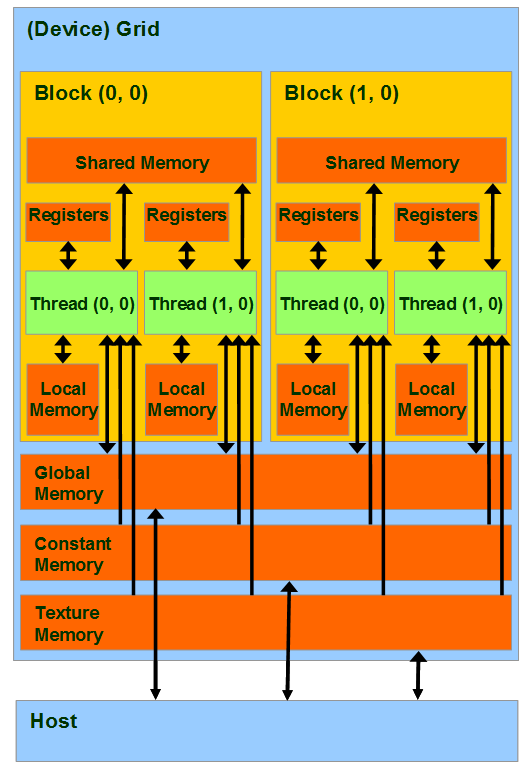
\includegraphics[width=0.5\textwidth]{memory.png}
      \caption{CUDA内存模型}
      \label{fig:chap2:slide}
    \end{figure}   

    共享内存得容量有限,通常为64KB。该存储空间位于流多处理器上类似于CPU的一级缓存,此内存空间被一个线程块中的
    所有线程共享。要合理的设置线程块的大小,避免因共享内存空间过度使用导致活跃线程束减少从而影响程序的执行效率。
    结合滑动窗的大小,我们最终将线程块的大小设置为8x8,将线程网格的大小设置为$(\left\lfloor {\frac{{w + 1}}{8}} \right\rfloor ,\left\lfloor {\frac{{h + 1}}{8}} \right\rfloor )$
    。其中$\left\lfloor {} \right\rfloor $代表向下取整,$w$代表SAR图像的宽度,$h$代表SAR图像的高度。
    
    在分配好线程块与线程网格大小后,每个线程与SAR图像像素索引对应关系为:row = threadIdx.x + blockDim.x * blockIdx.x; column = threadIdx.y + blockDim.y * blockIdx.y;
    之后根据滑动窗,将检测像素所对应的海杂波像素复制到该线程所对应的共享内存内存空间,在EM算法过程中在共享内存中读取杂波像素值进行分布
    的参数更新,当满足参数迭代停止条件后得到LMM分布参数,然后应用牛顿迭代法计算检测阈值$T$,当检测像素值大于阈值$T$时,
    该像素被标记为舰船目标像素。当所有线程执行完毕后,将检测结果从设备内存拷贝至主机内存,进行进一步的分析与处理。

    \begin{figure}[H] % use float package if you want it here
      \centering
      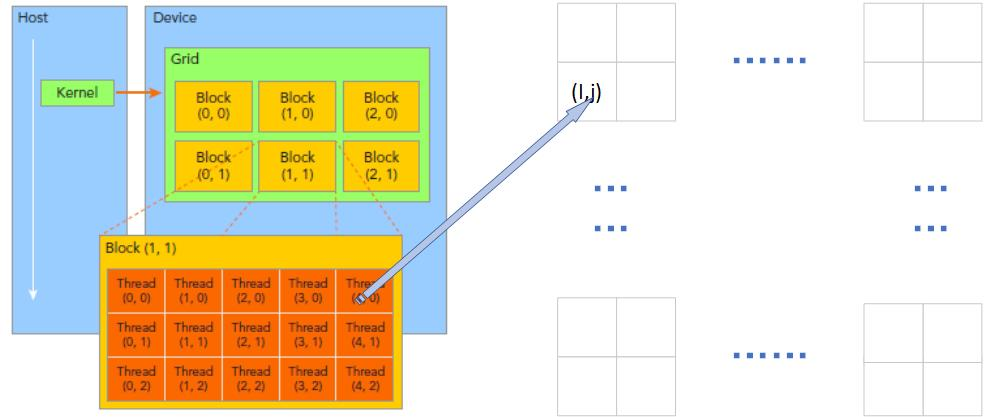
\includegraphics[width=0.9\textwidth]{map.jpg}
      \caption{CUDA线程与检测像素映射关系}
      \label{fig:chap2:slide}
    \end{figure} 

\section{LMM实验结果}
    本次实验中我们使用的是由星载成像雷达系统(SIR-C/X)拍摄的香港维多利亚港的SAR图像数据。SAR图像部分HH通道
    强度图像如图\ref{fig:chap2:source}所示


  \begin{figure}[h]
    \centering%
    \begin{subfigure}{0.4\textwidth}\
      \includegraphics[width=5cm]{HongKong1.png}
    \end{subfigure}%
    \begin{subfigure}{0.4\textwidth}
      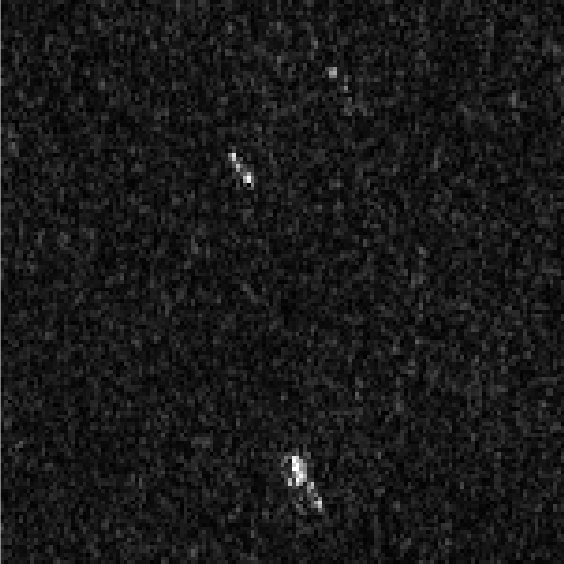
\includegraphics[width=5cm]{HongKong2.png}
    \end{subfigure}

    \begin{subfigure}{0.4\textwidth}
      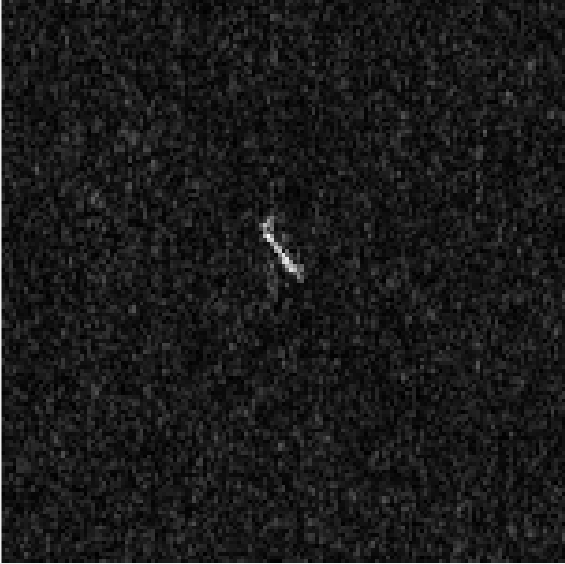
\includegraphics[height=5cm]{HongKong3.png}
    \end{subfigure}%
    \begin{subfigure}{0.4\textwidth}
      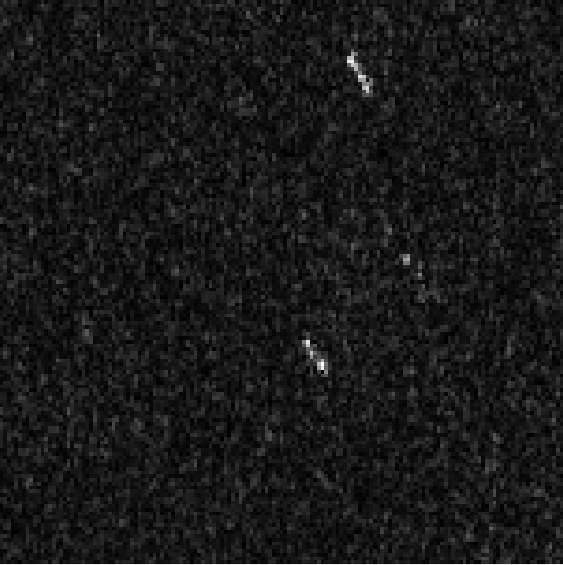
\includegraphics[height=5cm]{HongKong4.png}
    \end{subfigure}   

    \caption{四张SIR-C/XSAR强度图像}
    \label{fig:chap2:source}
  \end{figure}

  在检测中我们设置恒虚警为$1x10^{-5}$,检测结果如图\ref{fig:chap2:detectresult}所示,其中白色区域代表舰船目标像素区域,
  黑色区域代表背景杂波区域,从结果可以看出在给定的虚警率下LMM算法对目标像素与舰船像素作做出了正确的
  分割。本次实验使用的GPU为NVIDIA TITAN V,经过多次实验验证,相较于使用单线程CPU的检测方法,程序运行的时间效率提升了近21倍,
  不同平台运行时间如表所示,原始SAR图像中的舰船数量较少,检测结果中虚警漏报的数量均为0,准确率达到了$100\%$。

  \begin{figure}[h]
    \centering%
    \begin{subfigure}{0.4\textwidth}\
      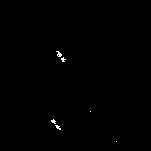
\includegraphics[width=5cm]{HongKong1r.jpg}
    \end{subfigure}%
    \begin{subfigure}{0.4\textwidth}
      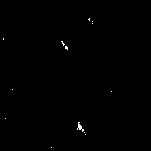
\includegraphics[width=5cm]{HongKong2r.jpg}
    \end{subfigure}

    \begin{subfigure}{0.4\textwidth}
      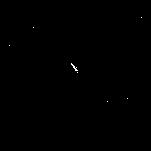
\includegraphics[height=5cm]{HongKong3r.jpg}
    \end{subfigure}%
    \begin{subfigure}{0.4\textwidth}
      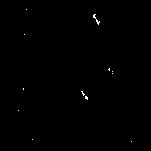
\includegraphics[height=5cm]{HongKong4r.jpg}
    \end{subfigure}   

    \caption{LMM检测结果}
    \label{fig:chap2:detectresult}
  \end{figure}

  \begin{table}[htb]
  \centering
    \begin{minipage}[t]{1\linewidth} % 如果想在表格中使用脚注,minipage是个不错的办法
    \caption[LMM算法时间]{串行与并行LMM算法运行时间对比}
    \label{tab:chap3:timeresult}
      \begin{tabularx}{\linewidth}{lXX}
        \toprule[1.5pt]
        {\heiti 检测算法} & {\heiti 运行平台} & {\heiti 运行时间/s} \\ \midrule[1pt]
        LMM-CFAR(Matlab单线程) & (Intel(R) i7-9750H CPU) & 15.1 \\
        LMM-CFAR(GPU多线程) &  GPU(Titan V) & 0.73 \\
        \bottomrule[1.5pt]
      \end{tabularx}
    \end{minipage}
  \end{table}

\section{小结}
    本章我们实现了基于混合对数正太分布的恒虚警率SAR图像舰船检测方法,在本质上混合对数分布等价于
    强度SAR图像在对数域上的混合高斯分布,因此采用了EM算法与牛顿迭代法得到分布参数与检测阈值。对于滑动窗
    参数估计的部分,我们将其放置在GPU上进行并行计算,并使用延迟更低的共享内存来加快访存速度。相较于传统的
    串行解决方案,本章基于GPU的LMM方法不仅在时间性能获得了显著的提升同时还保证了检测效果的有效性。


